% Created by tikzDevice version 0.6.2-92-0ad2792 on 2013-03-06 19:58:12
% !TEX encoding = UTF-8 Unicode
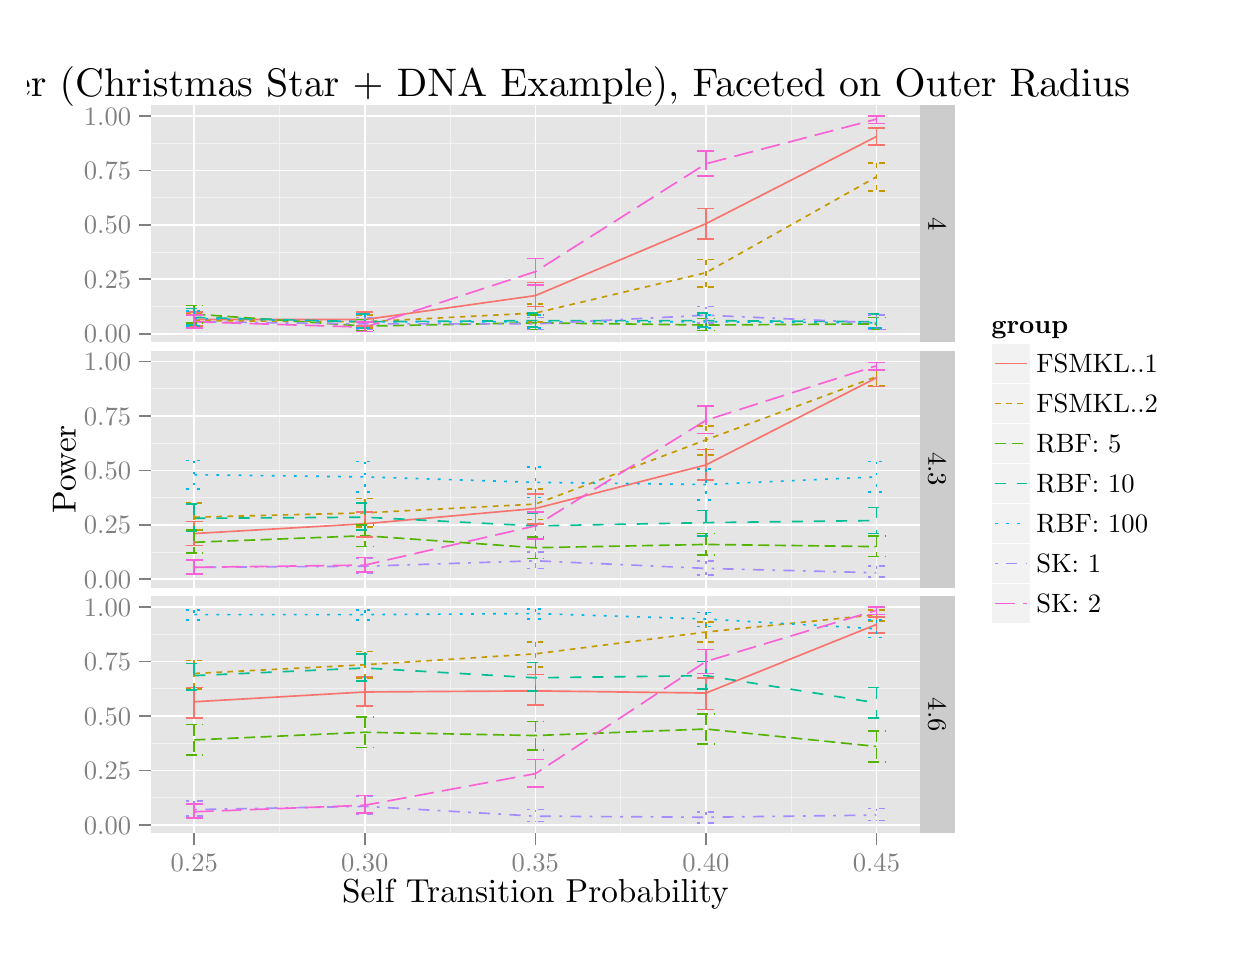
\begin{tikzpicture}[x=1pt,y=1pt]
\definecolor[named]{fillColor}{rgb}{1.00,1.00,1.00}
\path[use as bounding box,fill=fillColor,fill opacity=0.00] (0,0) rectangle (433.62,325.21);
\begin{scope}
\path[clip] (  0.00,  0.00) rectangle (433.62,325.21);
\definecolor[named]{drawColor}{rgb}{1.00,1.00,1.00}
\definecolor[named]{fillColor}{rgb}{1.00,1.00,1.00}

\path[draw=drawColor,line width= 0.6pt,line join=round,line cap=round,fill=fillColor] (  0.00,  0.00) rectangle (433.62,325.21);
\end{scope}
\begin{scope}
\path[clip] ( 44.49,211.51) rectangle (322.42,297.23);
\definecolor[named]{fillColor}{rgb}{0.90,0.90,0.90}

\path[fill=fillColor] ( 44.49,211.51) rectangle (322.42,297.23);
\definecolor[named]{drawColor}{rgb}{0.95,0.95,0.95}

\path[draw=drawColor,line width= 0.3pt,line join=round] ( 44.49,224.45) --
	(322.42,224.45);

\path[draw=drawColor,line width= 0.3pt,line join=round] ( 44.49,244.13) --
	(322.42,244.13);

\path[draw=drawColor,line width= 0.3pt,line join=round] ( 44.49,263.81) --
	(322.42,263.81);

\path[draw=drawColor,line width= 0.3pt,line join=round] ( 44.49,283.49) --
	(322.42,283.49);

\path[draw=drawColor,line width= 0.3pt,line join=round] ( 91.01,211.51) --
	( 91.01,297.23);

\path[draw=drawColor,line width= 0.3pt,line join=round] (152.64,211.51) --
	(152.64,297.23);

\path[draw=drawColor,line width= 0.3pt,line join=round] (214.27,211.51) --
	(214.27,297.23);

\path[draw=drawColor,line width= 0.3pt,line join=round] (275.89,211.51) --
	(275.89,297.23);
\definecolor[named]{drawColor}{rgb}{1.00,1.00,1.00}

\path[draw=drawColor,line width= 0.6pt,line join=round] ( 44.49,214.62) --
	(322.42,214.62);

\path[draw=drawColor,line width= 0.6pt,line join=round] ( 44.49,234.29) --
	(322.42,234.29);

\path[draw=drawColor,line width= 0.6pt,line join=round] ( 44.49,253.97) --
	(322.42,253.97);

\path[draw=drawColor,line width= 0.6pt,line join=round] ( 44.49,273.65) --
	(322.42,273.65);

\path[draw=drawColor,line width= 0.6pt,line join=round] ( 44.49,293.33) --
	(322.42,293.33);

\path[draw=drawColor,line width= 0.6pt,line join=round] ( 60.20,211.51) --
	( 60.20,297.23);

\path[draw=drawColor,line width= 0.6pt,line join=round] (121.83,211.51) --
	(121.83,297.23);

\path[draw=drawColor,line width= 0.6pt,line join=round] (183.45,211.51) --
	(183.45,297.23);

\path[draw=drawColor,line width= 0.6pt,line join=round] (245.08,211.51) --
	(245.08,297.23);

\path[draw=drawColor,line width= 0.6pt,line join=round] (306.70,211.51) --
	(306.70,297.23);
\definecolor[named]{drawColor}{rgb}{0.97,0.46,0.43}

\path[draw=drawColor,line width= 0.6pt,line join=round] ( 60.20,219.73) --
	(121.83,219.73) --
	(183.45,228.39) --
	(245.08,254.37) --
	(306.70,285.86);
\definecolor[named]{drawColor}{rgb}{0.77,0.60,0.00}

\path[draw=drawColor,line width= 0.6pt,dash pattern=on 2pt off 2pt ,line join=round] ( 60.20,219.34) --
	(121.83,218.94) --
	(183.45,222.09) --
	(245.08,236.66) --
	(306.70,271.29);
\definecolor[named]{drawColor}{rgb}{0.33,0.71,0.00}

\path[draw=drawColor,line width= 0.6pt,dash pattern=on 4pt off 2pt ,line join=round] ( 60.20,221.70) --
	(121.83,217.37) --
	(183.45,218.55) --
	(245.08,217.76) --
	(306.70,218.16);
\definecolor[named]{drawColor}{rgb}{0.00,0.75,0.58}

\path[draw=drawColor,line width= 0.6pt,dash pattern=on 4pt off 4pt ,line join=round] ( 60.20,220.52) --
	(121.83,218.94) --
	(183.45,219.34) --
	(245.08,219.34) --
	(306.70,218.94);
\definecolor[named]{drawColor}{rgb}{0.00,0.71,0.92}

\path[draw=drawColor,line width= 0.6pt,dash pattern=on 1pt off 3pt ,line join=round] ( 60.20,220.13) --
	(121.83,218.94) --
	(183.45,218.94) --
	(245.08,218.94) --
	(306.70,218.55);
\definecolor[named]{drawColor}{rgb}{0.65,0.54,1.00}

\path[draw=drawColor,line width= 0.6pt,dash pattern=on 1pt off 3pt on 4pt off 3pt ,line join=round] ( 60.20,218.94) --
	(121.83,218.16) --
	(183.45,218.16) --
	(245.08,221.31) --
	(306.70,218.55);
\definecolor[named]{drawColor}{rgb}{0.98,0.38,0.84}

\path[draw=drawColor,line width= 0.6pt,dash pattern=on 7pt off 3pt ,line join=round] ( 60.20,218.94) --
	(121.83,216.98) --
	(183.45,237.05) --
	(245.08,276.02) --
	(306.70,292.15);
\definecolor[named]{drawColor}{rgb}{0.97,0.46,0.43}

\path[draw=drawColor,line width= 0.6pt,line join=round] ( 57.12,222.49) --
	( 63.28,222.49);

\path[draw=drawColor,line width= 0.6pt,line join=round] ( 60.20,222.49) --
	( 60.20,217.36);

\path[draw=drawColor,line width= 0.6pt,line join=round] ( 57.12,217.36) --
	( 63.28,217.36);

\path[draw=drawColor,line width= 0.6pt,line join=round] (118.74,222.49) --
	(124.91,222.49);

\path[draw=drawColor,line width= 0.6pt,line join=round] (121.83,222.49) --
	(121.83,217.37);

\path[draw=drawColor,line width= 0.6pt,line join=round] (118.74,217.37) --
	(124.91,217.37);

\path[draw=drawColor,line width= 0.6pt,line join=round] (180.37,233.11) --
	(186.53,233.11);

\path[draw=drawColor,line width= 0.6pt,line join=round] (183.45,233.11) --
	(183.45,224.45);

\path[draw=drawColor,line width= 0.6pt,line join=round] (180.37,224.45) --
	(186.53,224.45);

\path[draw=drawColor,line width= 0.6pt,line join=round] (242.00,259.88) --
	(248.16,259.88);

\path[draw=drawColor,line width= 0.6pt,line join=round] (245.08,259.88) --
	(245.08,248.86);

\path[draw=drawColor,line width= 0.6pt,line join=round] (242.00,248.86) --
	(248.16,248.86);

\path[draw=drawColor,line width= 0.6pt,line join=round] (303.62,289.00) --
	(309.79,289.00);

\path[draw=drawColor,line width= 0.6pt,line join=round] (306.70,289.00) --
	(306.70,282.71);

\path[draw=drawColor,line width= 0.6pt,line join=round] (303.62,282.71) --
	(309.79,282.71);
\definecolor[named]{drawColor}{rgb}{0.77,0.60,0.00}

\path[draw=drawColor,line width= 0.6pt,dash pattern=on 2pt off 2pt ,line join=round] ( 57.12,221.70) --
	( 63.28,221.70);

\path[draw=drawColor,line width= 0.6pt,dash pattern=on 2pt off 2pt ,line join=round] ( 60.20,221.70) --
	( 60.20,216.98);

\path[draw=drawColor,line width= 0.6pt,dash pattern=on 2pt off 2pt ,line join=round] ( 57.12,216.98) --
	( 63.28,216.98);

\path[draw=drawColor,line width= 0.6pt,dash pattern=on 2pt off 2pt ,line join=round] (118.74,221.32) --
	(124.91,221.32);

\path[draw=drawColor,line width= 0.6pt,dash pattern=on 2pt off 2pt ,line join=round] (121.83,221.32) --
	(121.83,216.58);

\path[draw=drawColor,line width= 0.6pt,dash pattern=on 2pt off 2pt ,line join=round] (118.74,216.58) --
	(124.91,216.58);

\path[draw=drawColor,line width= 0.6pt,dash pattern=on 2pt off 2pt ,line join=round] (180.37,225.25) --
	(186.53,225.25);

\path[draw=drawColor,line width= 0.6pt,dash pattern=on 2pt off 2pt ,line join=round] (183.45,225.25) --
	(183.45,218.94);

\path[draw=drawColor,line width= 0.6pt,dash pattern=on 2pt off 2pt ,line join=round] (180.37,218.94) --
	(186.53,218.94);

\path[draw=drawColor,line width= 0.6pt,dash pattern=on 2pt off 2pt ,line join=round] (242.00,241.38) --
	(248.16,241.38);

\path[draw=drawColor,line width= 0.6pt,dash pattern=on 2pt off 2pt ,line join=round] (245.08,241.38) --
	(245.08,231.54);

\path[draw=drawColor,line width= 0.6pt,dash pattern=on 2pt off 2pt ,line join=round] (242.00,231.54) --
	(248.16,231.54);

\path[draw=drawColor,line width= 0.6pt,dash pattern=on 2pt off 2pt ,line join=round] (303.62,276.41) --
	(309.79,276.41);

\path[draw=drawColor,line width= 0.6pt,dash pattern=on 2pt off 2pt ,line join=round] (306.70,276.41) --
	(306.70,266.17);

\path[draw=drawColor,line width= 0.6pt,dash pattern=on 2pt off 2pt ,line join=round] (303.62,266.17) --
	(309.79,266.17);
\definecolor[named]{drawColor}{rgb}{0.33,0.71,0.00}

\path[draw=drawColor,line width= 0.6pt,dash pattern=on 4pt off 2pt ,line join=round] ( 57.12,224.85) --
	( 63.28,224.85);

\path[draw=drawColor,line width= 0.6pt,dash pattern=on 4pt off 2pt ,line join=round] ( 60.20,224.85) --
	( 60.20,218.55);

\path[draw=drawColor,line width= 0.6pt,dash pattern=on 4pt off 2pt ,line join=round] ( 57.12,218.55) --
	( 63.28,218.55);

\path[draw=drawColor,line width= 0.6pt,dash pattern=on 4pt off 2pt ,line join=round] (118.74,219.73) --
	(124.91,219.73);

\path[draw=drawColor,line width= 0.6pt,dash pattern=on 4pt off 2pt ,line join=round] (121.83,219.73) --
	(121.83,215.80);

\path[draw=drawColor,line width= 0.6pt,dash pattern=on 4pt off 2pt ,line join=round] (118.74,215.80) --
	(124.91,215.80);

\path[draw=drawColor,line width= 0.6pt,dash pattern=on 4pt off 2pt ,line join=round] (180.37,221.31) --
	(186.53,221.31);

\path[draw=drawColor,line width= 0.6pt,dash pattern=on 4pt off 2pt ,line join=round] (183.45,221.31) --
	(183.45,216.19);

\path[draw=drawColor,line width= 0.6pt,dash pattern=on 4pt off 2pt ,line join=round] (180.37,216.19) --
	(186.53,216.19);

\path[draw=drawColor,line width= 0.6pt,dash pattern=on 4pt off 2pt ,line join=round] (242.00,220.13) --
	(248.16,220.13);

\path[draw=drawColor,line width= 0.6pt,dash pattern=on 4pt off 2pt ,line join=round] (245.08,220.13) --
	(245.08,215.80);

\path[draw=drawColor,line width= 0.6pt,dash pattern=on 4pt off 2pt ,line join=round] (242.00,215.80) --
	(248.16,215.80);

\path[draw=drawColor,line width= 0.6pt,dash pattern=on 4pt off 2pt ,line join=round] (303.62,220.52) --
	(309.79,220.52);

\path[draw=drawColor,line width= 0.6pt,dash pattern=on 4pt off 2pt ,line join=round] (306.70,220.52) --
	(306.70,216.19);

\path[draw=drawColor,line width= 0.6pt,dash pattern=on 4pt off 2pt ,line join=round] (303.62,216.19) --
	(309.79,216.19);
\definecolor[named]{drawColor}{rgb}{0.00,0.75,0.58}

\path[draw=drawColor,line width= 0.6pt,dash pattern=on 4pt off 4pt ,line join=round] ( 57.12,223.67) --
	( 63.28,223.67);

\path[draw=drawColor,line width= 0.6pt,dash pattern=on 4pt off 4pt ,line join=round] ( 60.20,223.67) --
	( 60.20,217.76);

\path[draw=drawColor,line width= 0.6pt,dash pattern=on 4pt off 4pt ,line join=round] ( 57.12,217.76) --
	( 63.28,217.76);

\path[draw=drawColor,line width= 0.6pt,dash pattern=on 4pt off 4pt ,line join=round] (118.74,221.70) --
	(124.91,221.70);

\path[draw=drawColor,line width= 0.6pt,dash pattern=on 4pt off 4pt ,line join=round] (121.83,221.70) --
	(121.83,216.58);

\path[draw=drawColor,line width= 0.6pt,dash pattern=on 4pt off 4pt ,line join=round] (118.74,216.58) --
	(124.91,216.58);

\path[draw=drawColor,line width= 0.6pt,dash pattern=on 4pt off 4pt ,line join=round] (180.37,222.09) --
	(186.53,222.09);

\path[draw=drawColor,line width= 0.6pt,dash pattern=on 4pt off 4pt ,line join=round] (183.45,222.09) --
	(183.45,216.98);

\path[draw=drawColor,line width= 0.6pt,dash pattern=on 4pt off 4pt ,line join=round] (180.37,216.98) --
	(186.53,216.98);

\path[draw=drawColor,line width= 0.6pt,dash pattern=on 4pt off 4pt ,line join=round] (242.00,222.09) --
	(248.16,222.09);

\path[draw=drawColor,line width= 0.6pt,dash pattern=on 4pt off 4pt ,line join=round] (245.08,222.09) --
	(245.08,216.98);

\path[draw=drawColor,line width= 0.6pt,dash pattern=on 4pt off 4pt ,line join=round] (242.00,216.98) --
	(248.16,216.98);

\path[draw=drawColor,line width= 0.6pt,dash pattern=on 4pt off 4pt ,line join=round] (303.62,221.70) --
	(309.79,221.70);

\path[draw=drawColor,line width= 0.6pt,dash pattern=on 4pt off 4pt ,line join=round] (306.70,221.70) --
	(306.70,216.58);

\path[draw=drawColor,line width= 0.6pt,dash pattern=on 4pt off 4pt ,line join=round] (303.62,216.58) --
	(309.79,216.58);
\definecolor[named]{drawColor}{rgb}{0.00,0.71,0.92}

\path[draw=drawColor,line width= 0.6pt,dash pattern=on 1pt off 3pt ,line join=round] ( 57.12,222.88) --
	( 63.28,222.88);

\path[draw=drawColor,line width= 0.6pt,dash pattern=on 1pt off 3pt ,line join=round] ( 60.20,222.88) --
	( 60.20,217.37);

\path[draw=drawColor,line width= 0.6pt,dash pattern=on 1pt off 3pt ,line join=round] ( 57.12,217.37) --
	( 63.28,217.37);

\path[draw=drawColor,line width= 0.6pt,dash pattern=on 1pt off 3pt ,line join=round] (118.74,221.70) --
	(124.91,221.70);

\path[draw=drawColor,line width= 0.6pt,dash pattern=on 1pt off 3pt ,line join=round] (121.83,221.70) --
	(121.83,216.58);

\path[draw=drawColor,line width= 0.6pt,dash pattern=on 1pt off 3pt ,line join=round] (118.74,216.58) --
	(124.91,216.58);

\path[draw=drawColor,line width= 0.6pt,dash pattern=on 1pt off 3pt ,line join=round] (180.37,221.31) --
	(186.53,221.31);

\path[draw=drawColor,line width= 0.6pt,dash pattern=on 1pt off 3pt ,line join=round] (183.45,221.31) --
	(183.45,216.58);

\path[draw=drawColor,line width= 0.6pt,dash pattern=on 1pt off 3pt ,line join=round] (180.37,216.58) --
	(186.53,216.58);

\path[draw=drawColor,line width= 0.6pt,dash pattern=on 1pt off 3pt ,line join=round] (242.00,221.32) --
	(248.16,221.32);

\path[draw=drawColor,line width= 0.6pt,dash pattern=on 1pt off 3pt ,line join=round] (245.08,221.32) --
	(245.08,216.58);

\path[draw=drawColor,line width= 0.6pt,dash pattern=on 1pt off 3pt ,line join=round] (242.00,216.58) --
	(248.16,216.58);

\path[draw=drawColor,line width= 0.6pt,dash pattern=on 1pt off 3pt ,line join=round] (303.62,221.31) --
	(309.79,221.31);

\path[draw=drawColor,line width= 0.6pt,dash pattern=on 1pt off 3pt ,line join=round] (306.70,221.31) --
	(306.70,216.57);

\path[draw=drawColor,line width= 0.6pt,dash pattern=on 1pt off 3pt ,line join=round] (303.62,216.57) --
	(309.79,216.57);
\definecolor[named]{drawColor}{rgb}{0.65,0.54,1.00}

\path[draw=drawColor,line width= 0.6pt,dash pattern=on 1pt off 3pt on 4pt off 3pt ,line join=round] ( 57.12,221.32) --
	( 63.28,221.32);

\path[draw=drawColor,line width= 0.6pt,dash pattern=on 1pt off 3pt on 4pt off 3pt ,line join=round] ( 60.20,221.32) --
	( 60.20,216.58);

\path[draw=drawColor,line width= 0.6pt,dash pattern=on 1pt off 3pt on 4pt off 3pt ,line join=round] ( 57.12,216.58) --
	( 63.28,216.58);

\path[draw=drawColor,line width= 0.6pt,dash pattern=on 1pt off 3pt on 4pt off 3pt ,line join=round] (118.74,220.52) --
	(124.91,220.52);

\path[draw=drawColor,line width= 0.6pt,dash pattern=on 1pt off 3pt on 4pt off 3pt ,line join=round] (121.83,220.52) --
	(121.83,216.19);

\path[draw=drawColor,line width= 0.6pt,dash pattern=on 1pt off 3pt on 4pt off 3pt ,line join=round] (118.74,216.19) --
	(124.91,216.19);

\path[draw=drawColor,line width= 0.6pt,dash pattern=on 1pt off 3pt on 4pt off 3pt ,line join=round] (180.37,220.52) --
	(186.53,220.52);

\path[draw=drawColor,line width= 0.6pt,dash pattern=on 1pt off 3pt on 4pt off 3pt ,line join=round] (183.45,220.52) --
	(183.45,216.19);

\path[draw=drawColor,line width= 0.6pt,dash pattern=on 1pt off 3pt on 4pt off 3pt ,line join=round] (180.37,216.19) --
	(186.53,216.19);

\path[draw=drawColor,line width= 0.6pt,dash pattern=on 1pt off 3pt on 4pt off 3pt ,line join=round] (242.00,224.45) --
	(248.16,224.45);

\path[draw=drawColor,line width= 0.6pt,dash pattern=on 1pt off 3pt on 4pt off 3pt ,line join=round] (245.08,224.45) --
	(245.08,218.55);

\path[draw=drawColor,line width= 0.6pt,dash pattern=on 1pt off 3pt on 4pt off 3pt ,line join=round] (242.00,218.55) --
	(248.16,218.55);

\path[draw=drawColor,line width= 0.6pt,dash pattern=on 1pt off 3pt on 4pt off 3pt ,line join=round] (303.62,221.31) --
	(309.79,221.31);

\path[draw=drawColor,line width= 0.6pt,dash pattern=on 1pt off 3pt on 4pt off 3pt ,line join=round] (306.70,221.31) --
	(306.70,216.19);

\path[draw=drawColor,line width= 0.6pt,dash pattern=on 1pt off 3pt on 4pt off 3pt ,line join=round] (303.62,216.19) --
	(309.79,216.19);
\definecolor[named]{drawColor}{rgb}{0.98,0.38,0.84}

\path[draw=drawColor,line width= 0.6pt,dash pattern=on 7pt off 3pt ,line join=round] ( 57.12,221.31) --
	( 63.28,221.31);

\path[draw=drawColor,line width= 0.6pt,dash pattern=on 7pt off 3pt ,line join=round] ( 60.20,221.31) --
	( 60.20,216.58);

\path[draw=drawColor,line width= 0.6pt,dash pattern=on 7pt off 3pt ,line join=round] ( 57.12,216.58) --
	( 63.28,216.58);

\path[draw=drawColor,line width= 0.6pt,dash pattern=on 7pt off 3pt ,line join=round] (118.74,218.94) --
	(124.91,218.94);

\path[draw=drawColor,line width= 0.6pt,dash pattern=on 7pt off 3pt ,line join=round] (121.83,218.94) --
	(121.83,215.40);

\path[draw=drawColor,line width= 0.6pt,dash pattern=on 7pt off 3pt ,line join=round] (118.74,215.40) --
	(124.91,215.40);

\path[draw=drawColor,line width= 0.6pt,dash pattern=on 7pt off 3pt ,line join=round] (180.37,241.77) --
	(186.53,241.77);

\path[draw=drawColor,line width= 0.6pt,dash pattern=on 7pt off 3pt ,line join=round] (183.45,241.77) --
	(183.45,232.33);

\path[draw=drawColor,line width= 0.6pt,dash pattern=on 7pt off 3pt ,line join=round] (180.37,232.33) --
	(186.53,232.33);

\path[draw=drawColor,line width= 0.6pt,dash pattern=on 7pt off 3pt ,line join=round] (242.00,280.74) --
	(248.16,280.74);

\path[draw=drawColor,line width= 0.6pt,dash pattern=on 7pt off 3pt ,line join=round] (245.08,280.74) --
	(245.08,271.69);

\path[draw=drawColor,line width= 0.6pt,dash pattern=on 7pt off 3pt ,line join=round] (242.00,271.69) --
	(248.16,271.69);

\path[draw=drawColor,line width= 0.6pt,dash pattern=on 7pt off 3pt ,line join=round] (303.62,293.33) --
	(309.79,293.33);

\path[draw=drawColor,line width= 0.6pt,dash pattern=on 7pt off 3pt ,line join=round] (306.70,293.33) --
	(306.70,290.58);

\path[draw=drawColor,line width= 0.6pt,dash pattern=on 7pt off 3pt ,line join=round] (303.62,290.58) --
	(309.79,290.58);
\end{scope}
\begin{scope}
\path[clip] ( 44.49,122.77) rectangle (322.42,208.49);
\definecolor[named]{fillColor}{rgb}{0.90,0.90,0.90}

\path[fill=fillColor] ( 44.49,122.77) rectangle (322.42,208.49);
\definecolor[named]{drawColor}{rgb}{0.95,0.95,0.95}

\path[draw=drawColor,line width= 0.3pt,line join=round] ( 44.49,135.72) --
	(322.42,135.72);

\path[draw=drawColor,line width= 0.3pt,line join=round] ( 44.49,155.40) --
	(322.42,155.40);

\path[draw=drawColor,line width= 0.3pt,line join=round] ( 44.49,175.08) --
	(322.42,175.08);

\path[draw=drawColor,line width= 0.3pt,line join=round] ( 44.49,194.76) --
	(322.42,194.76);

\path[draw=drawColor,line width= 0.3pt,line join=round] ( 91.01,122.77) --
	( 91.01,208.49);

\path[draw=drawColor,line width= 0.3pt,line join=round] (152.64,122.77) --
	(152.64,208.49);

\path[draw=drawColor,line width= 0.3pt,line join=round] (214.27,122.77) --
	(214.27,208.49);

\path[draw=drawColor,line width= 0.3pt,line join=round] (275.89,122.77) --
	(275.89,208.49);
\definecolor[named]{drawColor}{rgb}{1.00,1.00,1.00}

\path[draw=drawColor,line width= 0.6pt,line join=round] ( 44.49,125.88) --
	(322.42,125.88);

\path[draw=drawColor,line width= 0.6pt,line join=round] ( 44.49,145.56) --
	(322.42,145.56);

\path[draw=drawColor,line width= 0.6pt,line join=round] ( 44.49,165.24) --
	(322.42,165.24);

\path[draw=drawColor,line width= 0.6pt,line join=round] ( 44.49,184.92) --
	(322.42,184.92);

\path[draw=drawColor,line width= 0.6pt,line join=round] ( 44.49,204.60) --
	(322.42,204.60);

\path[draw=drawColor,line width= 0.6pt,line join=round] ( 60.20,122.77) --
	( 60.20,208.49);

\path[draw=drawColor,line width= 0.6pt,line join=round] (121.83,122.77) --
	(121.83,208.49);

\path[draw=drawColor,line width= 0.6pt,line join=round] (183.45,122.77) --
	(183.45,208.49);

\path[draw=drawColor,line width= 0.6pt,line join=round] (245.08,122.77) --
	(245.08,208.49);

\path[draw=drawColor,line width= 0.6pt,line join=round] (306.70,122.77) --
	(306.70,208.49);
\definecolor[named]{drawColor}{rgb}{0.97,0.46,0.43}

\path[draw=drawColor,line width= 0.6pt,line join=round] ( 60.20,142.41) --
	(121.83,145.95) --
	(183.45,151.46) --
	(245.08,167.21) --
	(306.70,198.69);
\definecolor[named]{drawColor}{rgb}{0.77,0.60,0.00}

\path[draw=drawColor,line width= 0.6pt,dash pattern=on 2pt off 2pt ,line join=round] ( 60.20,148.31) --
	(121.83,149.89) --
	(183.45,153.04) --
	(245.08,176.26) --
	(306.70,199.09);
\definecolor[named]{drawColor}{rgb}{0.33,0.71,0.00}

\path[draw=drawColor,line width= 0.6pt,dash pattern=on 4pt off 2pt ,line join=round] ( 60.20,139.26) --
	(121.83,141.62) --
	(183.45,137.29) --
	(245.08,138.47) --
	(306.70,137.69);
\definecolor[named]{drawColor}{rgb}{0.00,0.75,0.58}

\path[draw=drawColor,line width= 0.6pt,dash pattern=on 4pt off 4pt ,line join=round] ( 60.20,147.92) --
	(121.83,148.31) --
	(183.45,145.17) --
	(245.08,146.35) --
	(306.70,147.13);
\definecolor[named]{drawColor}{rgb}{0.00,0.71,0.92}

\path[draw=drawColor,line width= 0.6pt,dash pattern=on 1pt off 3pt ,line join=round] ( 60.20,163.66) --
	(121.83,162.88) --
	(183.45,160.91) --
	(245.08,160.12) --
	(306.70,162.88);
\definecolor[named]{drawColor}{rgb}{0.65,0.54,1.00}

\path[draw=drawColor,line width= 0.6pt,dash pattern=on 1pt off 3pt on 4pt off 3pt ,line join=round] ( 60.20,130.21) --
	(121.83,130.60) --
	(183.45,132.57) --
	(245.08,129.82) --
	(306.70,128.24);
\definecolor[named]{drawColor}{rgb}{0.98,0.38,0.84}

\path[draw=drawColor,line width= 0.6pt,dash pattern=on 7pt off 3pt ,line join=round] ( 60.20,130.21) --
	(121.83,131.00) --
	(183.45,145.17) --
	(245.08,183.34) --
	(306.70,203.02);
\definecolor[named]{drawColor}{rgb}{0.97,0.46,0.43}

\path[draw=drawColor,line width= 0.6pt,line join=round] ( 57.12,146.74) --
	( 63.28,146.74);

\path[draw=drawColor,line width= 0.6pt,line join=round] ( 60.20,146.74) --
	( 60.20,138.08);

\path[draw=drawColor,line width= 0.6pt,line join=round] ( 57.12,138.08) --
	( 63.28,138.08);

\path[draw=drawColor,line width= 0.6pt,line join=round] (118.74,150.28) --
	(124.91,150.28);

\path[draw=drawColor,line width= 0.6pt,line join=round] (121.83,150.28) --
	(121.83,141.23);

\path[draw=drawColor,line width= 0.6pt,line join=round] (118.74,141.23) --
	(124.91,141.23);

\path[draw=drawColor,line width= 0.6pt,line join=round] (180.37,156.59) --
	(186.53,156.59);

\path[draw=drawColor,line width= 0.6pt,line join=round] (183.45,156.59) --
	(183.45,145.95);

\path[draw=drawColor,line width= 0.6pt,line join=round] (180.37,145.95) --
	(186.53,145.95);

\path[draw=drawColor,line width= 0.6pt,line join=round] (242.00,172.73) --
	(248.16,172.73);

\path[draw=drawColor,line width= 0.6pt,line join=round] (245.08,172.73) --
	(245.08,161.69);

\path[draw=drawColor,line width= 0.6pt,line join=round] (242.00,161.69) --
	(248.16,161.69);

\path[draw=drawColor,line width= 0.6pt,line join=round] (303.62,201.45) --
	(309.79,201.45);

\path[draw=drawColor,line width= 0.6pt,line join=round] (306.70,201.45) --
	(306.70,195.55);

\path[draw=drawColor,line width= 0.6pt,line join=round] (303.62,195.55) --
	(309.79,195.55);
\definecolor[named]{drawColor}{rgb}{0.77,0.60,0.00}

\path[draw=drawColor,line width= 0.6pt,dash pattern=on 2pt off 2pt ,line join=round] ( 57.12,153.43) --
	( 63.28,153.43);

\path[draw=drawColor,line width= 0.6pt,dash pattern=on 2pt off 2pt ,line join=round] ( 60.20,153.43) --
	( 60.20,143.59);

\path[draw=drawColor,line width= 0.6pt,dash pattern=on 2pt off 2pt ,line join=round] ( 57.12,143.59) --
	( 63.28,143.59);

\path[draw=drawColor,line width= 0.6pt,dash pattern=on 2pt off 2pt ,line join=round] (118.74,155.02) --
	(124.91,155.02);

\path[draw=drawColor,line width= 0.6pt,dash pattern=on 2pt off 2pt ,line join=round] (121.83,155.02) --
	(121.83,144.77);

\path[draw=drawColor,line width= 0.6pt,dash pattern=on 2pt off 2pt ,line join=round] (118.74,144.77) --
	(124.91,144.77);

\path[draw=drawColor,line width= 0.6pt,dash pattern=on 2pt off 2pt ,line join=round] (180.37,158.55) --
	(186.53,158.55);

\path[draw=drawColor,line width= 0.6pt,dash pattern=on 2pt off 2pt ,line join=round] (183.45,158.55) --
	(183.45,147.53);

\path[draw=drawColor,line width= 0.6pt,dash pattern=on 2pt off 2pt ,line join=round] (180.37,147.53) --
	(186.53,147.53);

\path[draw=drawColor,line width= 0.6pt,dash pattern=on 2pt off 2pt ,line join=round] (242.00,181.38) --
	(248.16,181.38);

\path[draw=drawColor,line width= 0.6pt,dash pattern=on 2pt off 2pt ,line join=round] (245.08,181.38) --
	(245.08,170.75);

\path[draw=drawColor,line width= 0.6pt,dash pattern=on 2pt off 2pt ,line join=round] (242.00,170.75) --
	(248.16,170.75);

\path[draw=drawColor,line width= 0.6pt,dash pattern=on 2pt off 2pt ,line join=round] (303.62,201.45) --
	(309.79,201.45);

\path[draw=drawColor,line width= 0.6pt,dash pattern=on 2pt off 2pt ,line join=round] (306.70,201.45) --
	(306.70,195.94);

\path[draw=drawColor,line width= 0.6pt,dash pattern=on 2pt off 2pt ,line join=round] (303.62,195.94) --
	(309.79,195.94);
\definecolor[named]{drawColor}{rgb}{0.33,0.71,0.00}

\path[draw=drawColor,line width= 0.6pt,dash pattern=on 4pt off 2pt ,line join=round] ( 57.12,143.59) --
	( 63.28,143.59);

\path[draw=drawColor,line width= 0.6pt,dash pattern=on 4pt off 2pt ,line join=round] ( 60.20,143.59) --
	( 60.20,135.33);

\path[draw=drawColor,line width= 0.6pt,dash pattern=on 4pt off 2pt ,line join=round] ( 57.12,135.33) --
	( 63.28,135.33);

\path[draw=drawColor,line width= 0.6pt,dash pattern=on 4pt off 2pt ,line join=round] (118.74,145.57) --
	(124.91,145.57);

\path[draw=drawColor,line width= 0.6pt,dash pattern=on 4pt off 2pt ,line join=round] (121.83,145.57) --
	(121.83,137.69);

\path[draw=drawColor,line width= 0.6pt,dash pattern=on 4pt off 2pt ,line join=round] (118.74,137.69) --
	(124.91,137.69);

\path[draw=drawColor,line width= 0.6pt,dash pattern=on 4pt off 2pt ,line join=round] (180.37,141.23) --
	(186.53,141.23);

\path[draw=drawColor,line width= 0.6pt,dash pattern=on 4pt off 2pt ,line join=round] (183.45,141.23) --
	(183.45,133.36);

\path[draw=drawColor,line width= 0.6pt,dash pattern=on 4pt off 2pt ,line join=round] (180.37,133.36) --
	(186.53,133.36);

\path[draw=drawColor,line width= 0.6pt,dash pattern=on 4pt off 2pt ,line join=round] (242.00,142.42) --
	(248.16,142.42);

\path[draw=drawColor,line width= 0.6pt,dash pattern=on 4pt off 2pt ,line join=round] (245.08,142.42) --
	(245.08,134.54);

\path[draw=drawColor,line width= 0.6pt,dash pattern=on 4pt off 2pt ,line join=round] (242.00,134.54) --
	(248.16,134.54);

\path[draw=drawColor,line width= 0.6pt,dash pattern=on 4pt off 2pt ,line join=round] (303.62,141.62) --
	(309.79,141.62);

\path[draw=drawColor,line width= 0.6pt,dash pattern=on 4pt off 2pt ,line join=round] (306.70,141.62) --
	(306.70,134.14);

\path[draw=drawColor,line width= 0.6pt,dash pattern=on 4pt off 2pt ,line join=round] (303.62,134.14) --
	(309.79,134.14);
\definecolor[named]{drawColor}{rgb}{0.00,0.75,0.58}

\path[draw=drawColor,line width= 0.6pt,dash pattern=on 4pt off 4pt ,line join=round] ( 57.12,153.04) --
	( 63.28,153.04);

\path[draw=drawColor,line width= 0.6pt,dash pattern=on 4pt off 4pt ,line join=round] ( 60.20,153.04) --
	( 60.20,143.20);

\path[draw=drawColor,line width= 0.6pt,dash pattern=on 4pt off 4pt ,line join=round] ( 57.12,143.20) --
	( 63.28,143.20);

\path[draw=drawColor,line width= 0.6pt,dash pattern=on 4pt off 4pt ,line join=round] (118.74,153.43) --
	(124.91,153.43);

\path[draw=drawColor,line width= 0.6pt,dash pattern=on 4pt off 4pt ,line join=round] (121.83,153.43) --
	(121.83,143.59);

\path[draw=drawColor,line width= 0.6pt,dash pattern=on 4pt off 4pt ,line join=round] (118.74,143.59) --
	(124.91,143.59);

\path[draw=drawColor,line width= 0.6pt,dash pattern=on 4pt off 4pt ,line join=round] (180.37,149.89) --
	(186.53,149.89);

\path[draw=drawColor,line width= 0.6pt,dash pattern=on 4pt off 4pt ,line join=round] (183.45,149.89) --
	(183.45,140.44);

\path[draw=drawColor,line width= 0.6pt,dash pattern=on 4pt off 4pt ,line join=round] (180.37,140.44) --
	(186.53,140.44);

\path[draw=drawColor,line width= 0.6pt,dash pattern=on 4pt off 4pt ,line join=round] (242.00,150.68) --
	(248.16,150.68);

\path[draw=drawColor,line width= 0.6pt,dash pattern=on 4pt off 4pt ,line join=round] (245.08,150.68) --
	(245.08,141.62);

\path[draw=drawColor,line width= 0.6pt,dash pattern=on 4pt off 4pt ,line join=round] (242.00,141.62) --
	(248.16,141.62);

\path[draw=drawColor,line width= 0.6pt,dash pattern=on 4pt off 4pt ,line join=round] (303.62,151.86) --
	(309.79,151.86);

\path[draw=drawColor,line width= 0.6pt,dash pattern=on 4pt off 4pt ,line join=round] (306.70,151.86) --
	(306.70,142.40);

\path[draw=drawColor,line width= 0.6pt,dash pattern=on 4pt off 4pt ,line join=round] (303.62,142.40) --
	(309.79,142.40);
\definecolor[named]{drawColor}{rgb}{0.00,0.71,0.92}

\path[draw=drawColor,line width= 0.6pt,dash pattern=on 1pt off 3pt ,line join=round] ( 57.12,168.78) --
	( 63.28,168.78);

\path[draw=drawColor,line width= 0.6pt,dash pattern=on 1pt off 3pt ,line join=round] ( 60.20,168.78) --
	( 60.20,158.54);

\path[draw=drawColor,line width= 0.6pt,dash pattern=on 1pt off 3pt ,line join=round] ( 57.12,158.54) --
	( 63.28,158.54);

\path[draw=drawColor,line width= 0.6pt,dash pattern=on 1pt off 3pt ,line join=round] (118.74,168.39) --
	(124.91,168.39);

\path[draw=drawColor,line width= 0.6pt,dash pattern=on 1pt off 3pt ,line join=round] (121.83,168.39) --
	(121.83,157.37);

\path[draw=drawColor,line width= 0.6pt,dash pattern=on 1pt off 3pt ,line join=round] (118.74,157.37) --
	(124.91,157.37);

\path[draw=drawColor,line width= 0.6pt,dash pattern=on 1pt off 3pt ,line join=round] (180.37,166.42) --
	(186.53,166.42);

\path[draw=drawColor,line width= 0.6pt,dash pattern=on 1pt off 3pt ,line join=round] (183.45,166.42) --
	(183.45,155.40);

\path[draw=drawColor,line width= 0.6pt,dash pattern=on 1pt off 3pt ,line join=round] (180.37,155.40) --
	(186.53,155.40);

\path[draw=drawColor,line width= 0.6pt,dash pattern=on 1pt off 3pt ,line join=round] (242.00,165.63) --
	(248.16,165.63);

\path[draw=drawColor,line width= 0.6pt,dash pattern=on 1pt off 3pt ,line join=round] (245.08,165.63) --
	(245.08,154.61);

\path[draw=drawColor,line width= 0.6pt,dash pattern=on 1pt off 3pt ,line join=round] (242.00,154.61) --
	(248.16,154.61);

\path[draw=drawColor,line width= 0.6pt,dash pattern=on 1pt off 3pt ,line join=round] (303.62,168.39) --
	(309.79,168.39);

\path[draw=drawColor,line width= 0.6pt,dash pattern=on 1pt off 3pt ,line join=round] (306.70,168.39) --
	(306.70,157.37);

\path[draw=drawColor,line width= 0.6pt,dash pattern=on 1pt off 3pt ,line join=round] (303.62,157.37) --
	(309.79,157.37);
\definecolor[named]{drawColor}{rgb}{0.65,0.54,1.00}

\path[draw=drawColor,line width= 0.6pt,dash pattern=on 1pt off 3pt on 4pt off 3pt ,line join=round] ( 57.12,132.96) --
	( 63.28,132.96);

\path[draw=drawColor,line width= 0.6pt,dash pattern=on 1pt off 3pt on 4pt off 3pt ,line join=round] ( 60.20,132.96) --
	( 60.20,127.85);

\path[draw=drawColor,line width= 0.6pt,dash pattern=on 1pt off 3pt on 4pt off 3pt ,line join=round] ( 57.12,127.85) --
	( 63.28,127.85);

\path[draw=drawColor,line width= 0.6pt,dash pattern=on 1pt off 3pt on 4pt off 3pt ,line join=round] (118.74,133.36) --
	(124.91,133.36);

\path[draw=drawColor,line width= 0.6pt,dash pattern=on 1pt off 3pt on 4pt off 3pt ,line join=round] (121.83,133.36) --
	(121.83,128.24);

\path[draw=drawColor,line width= 0.6pt,dash pattern=on 1pt off 3pt on 4pt off 3pt ,line join=round] (118.74,128.24) --
	(124.91,128.24);

\path[draw=drawColor,line width= 0.6pt,dash pattern=on 1pt off 3pt on 4pt off 3pt ,line join=round] (180.37,135.72) --
	(186.53,135.72);

\path[draw=drawColor,line width= 0.6pt,dash pattern=on 1pt off 3pt on 4pt off 3pt ,line join=round] (183.45,135.72) --
	(183.45,129.82);

\path[draw=drawColor,line width= 0.6pt,dash pattern=on 1pt off 3pt on 4pt off 3pt ,line join=round] (180.37,129.82) --
	(186.53,129.82);

\path[draw=drawColor,line width= 0.6pt,dash pattern=on 1pt off 3pt on 4pt off 3pt ,line join=round] (242.00,132.57) --
	(248.16,132.57);

\path[draw=drawColor,line width= 0.6pt,dash pattern=on 1pt off 3pt on 4pt off 3pt ,line join=round] (245.08,132.57) --
	(245.08,127.45);

\path[draw=drawColor,line width= 0.6pt,dash pattern=on 1pt off 3pt on 4pt off 3pt ,line join=round] (242.00,127.45) --
	(248.16,127.45);

\path[draw=drawColor,line width= 0.6pt,dash pattern=on 1pt off 3pt on 4pt off 3pt ,line join=round] (303.62,130.60) --
	(309.79,130.60);

\path[draw=drawColor,line width= 0.6pt,dash pattern=on 1pt off 3pt on 4pt off 3pt ,line join=round] (306.70,130.60) --
	(306.70,126.67);

\path[draw=drawColor,line width= 0.6pt,dash pattern=on 1pt off 3pt on 4pt off 3pt ,line join=round] (303.62,126.67) --
	(309.79,126.67);
\definecolor[named]{drawColor}{rgb}{0.98,0.38,0.84}

\path[draw=drawColor,line width= 0.6pt,dash pattern=on 7pt off 3pt ,line join=round] ( 57.12,132.96) --
	( 63.28,132.96);

\path[draw=drawColor,line width= 0.6pt,dash pattern=on 7pt off 3pt ,line join=round] ( 60.20,132.96) --
	( 60.20,127.85);

\path[draw=drawColor,line width= 0.6pt,dash pattern=on 7pt off 3pt ,line join=round] ( 57.12,127.85) --
	( 63.28,127.85);

\path[draw=drawColor,line width= 0.6pt,dash pattern=on 7pt off 3pt ,line join=round] (118.74,133.75) --
	(124.91,133.75);

\path[draw=drawColor,line width= 0.6pt,dash pattern=on 7pt off 3pt ,line join=round] (121.83,133.75) --
	(121.83,128.62);

\path[draw=drawColor,line width= 0.6pt,dash pattern=on 7pt off 3pt ,line join=round] (118.74,128.62) --
	(124.91,128.62);

\path[draw=drawColor,line width= 0.6pt,dash pattern=on 7pt off 3pt ,line join=round] (180.37,150.28) --
	(186.53,150.28);

\path[draw=drawColor,line width= 0.6pt,dash pattern=on 7pt off 3pt ,line join=round] (183.45,150.28) --
	(183.45,140.44);

\path[draw=drawColor,line width= 0.6pt,dash pattern=on 7pt off 3pt ,line join=round] (180.37,140.44) --
	(186.53,140.44);

\path[draw=drawColor,line width= 0.6pt,dash pattern=on 7pt off 3pt ,line join=round] (242.00,188.46) --
	(248.16,188.46);

\path[draw=drawColor,line width= 0.6pt,dash pattern=on 7pt off 3pt ,line join=round] (245.08,188.46) --
	(245.08,178.62);

\path[draw=drawColor,line width= 0.6pt,dash pattern=on 7pt off 3pt ,line join=round] (242.00,178.62) --
	(248.16,178.62);

\path[draw=drawColor,line width= 0.6pt,dash pattern=on 7pt off 3pt ,line join=round] (303.62,204.20) --
	(309.79,204.20);

\path[draw=drawColor,line width= 0.6pt,dash pattern=on 7pt off 3pt ,line join=round] (306.70,204.20) --
	(306.70,201.45);

\path[draw=drawColor,line width= 0.6pt,dash pattern=on 7pt off 3pt ,line join=round] (303.62,201.45) --
	(309.79,201.45);
\end{scope}
\begin{scope}
\path[clip] ( 44.49, 34.03) rectangle (322.42,119.76);
\definecolor[named]{fillColor}{rgb}{0.90,0.90,0.90}

\path[fill=fillColor] ( 44.49, 34.03) rectangle (322.42,119.76);
\definecolor[named]{drawColor}{rgb}{0.95,0.95,0.95}

\path[draw=drawColor,line width= 0.3pt,line join=round] ( 44.49, 46.98) --
	(322.42, 46.98);

\path[draw=drawColor,line width= 0.3pt,line join=round] ( 44.49, 66.66) --
	(322.42, 66.66);

\path[draw=drawColor,line width= 0.3pt,line join=round] ( 44.49, 86.34) --
	(322.42, 86.34);

\path[draw=drawColor,line width= 0.3pt,line join=round] ( 44.49,106.02) --
	(322.42,106.02);

\path[draw=drawColor,line width= 0.3pt,line join=round] ( 91.01, 34.03) --
	( 91.01,119.76);

\path[draw=drawColor,line width= 0.3pt,line join=round] (152.64, 34.03) --
	(152.64,119.76);

\path[draw=drawColor,line width= 0.3pt,line join=round] (214.27, 34.03) --
	(214.27,119.76);

\path[draw=drawColor,line width= 0.3pt,line join=round] (275.89, 34.03) --
	(275.89,119.76);
\definecolor[named]{drawColor}{rgb}{1.00,1.00,1.00}

\path[draw=drawColor,line width= 0.6pt,line join=round] ( 44.49, 37.14) --
	(322.42, 37.14);

\path[draw=drawColor,line width= 0.6pt,line join=round] ( 44.49, 56.82) --
	(322.42, 56.82);

\path[draw=drawColor,line width= 0.6pt,line join=round] ( 44.49, 76.50) --
	(322.42, 76.50);

\path[draw=drawColor,line width= 0.6pt,line join=round] ( 44.49, 96.18) --
	(322.42, 96.18);

\path[draw=drawColor,line width= 0.6pt,line join=round] ( 44.49,115.86) --
	(322.42,115.86);

\path[draw=drawColor,line width= 0.6pt,line join=round] ( 60.20, 34.03) --
	( 60.20,119.76);

\path[draw=drawColor,line width= 0.6pt,line join=round] (121.83, 34.03) --
	(121.83,119.76);

\path[draw=drawColor,line width= 0.6pt,line join=round] (183.45, 34.03) --
	(183.45,119.76);

\path[draw=drawColor,line width= 0.6pt,line join=round] (245.08, 34.03) --
	(245.08,119.76);

\path[draw=drawColor,line width= 0.6pt,line join=round] (306.70, 34.03) --
	(306.70,119.76);
\definecolor[named]{drawColor}{rgb}{0.97,0.46,0.43}

\path[draw=drawColor,line width= 0.6pt,line join=round] ( 60.20, 81.62) --
	(121.83, 85.16) --
	(183.45, 85.56) --
	(245.08, 84.77) --
	(306.70,109.56);
\definecolor[named]{drawColor}{rgb}{0.77,0.60,0.00}

\path[draw=drawColor,line width= 0.6pt,dash pattern=on 2pt off 2pt ,line join=round] ( 60.20, 91.85) --
	(121.83, 95.00) --
	(183.45, 98.94) --
	(245.08,106.81) --
	(306.70,113.11);
\definecolor[named]{drawColor}{rgb}{0.33,0.71,0.00}

\path[draw=drawColor,line width= 0.6pt,dash pattern=on 4pt off 2pt ,line join=round] ( 60.20, 67.84) --
	(121.83, 70.60) --
	(183.45, 69.42) --
	(245.08, 71.78) --
	(306.70, 65.48);
\definecolor[named]{drawColor}{rgb}{0.00,0.75,0.58}

\path[draw=drawColor,line width= 0.6pt,dash pattern=on 4pt off 4pt ,line join=round] ( 60.20, 91.07) --
	(121.83, 93.82) --
	(183.45, 90.28) --
	(245.08, 91.07) --
	(306.70, 81.23);
\definecolor[named]{drawColor}{rgb}{0.00,0.71,0.92}

\path[draw=drawColor,line width= 0.6pt,dash pattern=on 1pt off 3pt ,line join=round] ( 60.20,113.11) --
	(121.83,113.11) --
	(183.45,113.50) --
	(245.08,111.53) --
	(306.70,107.99);
\definecolor[named]{drawColor}{rgb}{0.65,0.54,1.00}

\path[draw=drawColor,line width= 0.6pt,dash pattern=on 1pt off 3pt on 4pt off 3pt ,line join=round] ( 60.20, 42.65) --
	(121.83, 43.84) --
	(183.45, 40.29) --
	(245.08, 39.90) --
	(306.70, 40.69);
\definecolor[named]{drawColor}{rgb}{0.98,0.38,0.84}

\path[draw=drawColor,line width= 0.6pt,dash pattern=on 7pt off 3pt ,line join=round] ( 60.20, 41.87) --
	(121.83, 44.23) --
	(183.45, 55.64) --
	(245.08, 96.18) --
	(306.70,114.68);
\definecolor[named]{drawColor}{rgb}{0.97,0.46,0.43}

\path[draw=drawColor,line width= 0.6pt,line join=round] ( 57.12, 86.74) --
	( 63.28, 86.74);

\path[draw=drawColor,line width= 0.6pt,line join=round] ( 60.20, 86.74) --
	( 60.20, 75.72);

\path[draw=drawColor,line width= 0.6pt,line join=round] ( 57.12, 75.72) --
	( 63.28, 75.72);

\path[draw=drawColor,line width= 0.6pt,line join=round] (118.74, 90.67) --
	(124.91, 90.67);

\path[draw=drawColor,line width= 0.6pt,line join=round] (121.83, 90.67) --
	(121.83, 80.05);

\path[draw=drawColor,line width= 0.6pt,line join=round] (118.74, 80.05) --
	(124.91, 80.05);

\path[draw=drawColor,line width= 0.6pt,line join=round] (180.37, 91.46) --
	(186.53, 91.46);

\path[draw=drawColor,line width= 0.6pt,line join=round] (183.45, 91.46) --
	(183.45, 80.44);

\path[draw=drawColor,line width= 0.6pt,line join=round] (180.37, 80.44) --
	(186.53, 80.44);

\path[draw=drawColor,line width= 0.6pt,line join=round] (242.00, 90.28) --
	(248.16, 90.28);

\path[draw=drawColor,line width= 0.6pt,line join=round] (245.08, 90.28) --
	(245.08, 78.86);

\path[draw=drawColor,line width= 0.6pt,line join=round] (242.00, 78.86) --
	(248.16, 78.86);

\path[draw=drawColor,line width= 0.6pt,line join=round] (303.62,112.32) --
	(309.79,112.32);

\path[draw=drawColor,line width= 0.6pt,line join=round] (306.70,112.32) --
	(306.70,106.42);

\path[draw=drawColor,line width= 0.6pt,line join=round] (303.62,106.42) --
	(309.79,106.42);
\definecolor[named]{drawColor}{rgb}{0.77,0.60,0.00}

\path[draw=drawColor,line width= 0.6pt,dash pattern=on 2pt off 2pt ,line join=round] ( 57.12, 96.58) --
	( 63.28, 96.58);

\path[draw=drawColor,line width= 0.6pt,dash pattern=on 2pt off 2pt ,line join=round] ( 60.20, 96.58) --
	( 60.20, 86.34);

\path[draw=drawColor,line width= 0.6pt,dash pattern=on 2pt off 2pt ,line join=round] ( 57.12, 86.34) --
	( 63.28, 86.34);

\path[draw=drawColor,line width= 0.6pt,dash pattern=on 2pt off 2pt ,line join=round] (118.74, 99.73) --
	(124.91, 99.73);

\path[draw=drawColor,line width= 0.6pt,dash pattern=on 2pt off 2pt ,line join=round] (121.83, 99.73) --
	(121.83, 90.28);

\path[draw=drawColor,line width= 0.6pt,dash pattern=on 2pt off 2pt ,line join=round] (118.74, 90.28) --
	(124.91, 90.28);

\path[draw=drawColor,line width= 0.6pt,dash pattern=on 2pt off 2pt ,line join=round] (180.37,103.27) --
	(186.53,103.27);

\path[draw=drawColor,line width= 0.6pt,dash pattern=on 2pt off 2pt ,line join=round] (183.45,103.27) --
	(183.45, 94.21);

\path[draw=drawColor,line width= 0.6pt,dash pattern=on 2pt off 2pt ,line join=round] (180.37, 94.21) --
	(186.53, 94.21);

\path[draw=drawColor,line width= 0.6pt,dash pattern=on 2pt off 2pt ,line join=round] (242.00,110.35) --
	(248.16,110.35);

\path[draw=drawColor,line width= 0.6pt,dash pattern=on 2pt off 2pt ,line join=round] (245.08,110.35) --
	(245.08,103.27);

\path[draw=drawColor,line width= 0.6pt,dash pattern=on 2pt off 2pt ,line join=round] (242.00,103.27) --
	(248.16,103.27);

\path[draw=drawColor,line width= 0.6pt,dash pattern=on 2pt off 2pt ,line join=round] (303.62,114.68) --
	(309.79,114.68);

\path[draw=drawColor,line width= 0.6pt,dash pattern=on 2pt off 2pt ,line join=round] (306.70,114.68) --
	(306.70,110.75);

\path[draw=drawColor,line width= 0.6pt,dash pattern=on 2pt off 2pt ,line join=round] (303.62,110.75) --
	(309.79,110.75);
\definecolor[named]{drawColor}{rgb}{0.33,0.71,0.00}

\path[draw=drawColor,line width= 0.6pt,dash pattern=on 4pt off 2pt ,line join=round] ( 57.12, 73.35) --
	( 63.28, 73.35);

\path[draw=drawColor,line width= 0.6pt,dash pattern=on 4pt off 2pt ,line join=round] ( 60.20, 73.35) --
	( 60.20, 62.33);

\path[draw=drawColor,line width= 0.6pt,dash pattern=on 4pt off 2pt ,line join=round] ( 57.12, 62.33) --
	( 63.28, 62.33);

\path[draw=drawColor,line width= 0.6pt,dash pattern=on 4pt off 2pt ,line join=round] (118.74, 76.11) --
	(124.91, 76.11);

\path[draw=drawColor,line width= 0.6pt,dash pattern=on 4pt off 2pt ,line join=round] (121.83, 76.11) --
	(121.83, 65.09);

\path[draw=drawColor,line width= 0.6pt,dash pattern=on 4pt off 2pt ,line join=round] (118.74, 65.09) --
	(124.91, 65.09);

\path[draw=drawColor,line width= 0.6pt,dash pattern=on 4pt off 2pt ,line join=round] (180.37, 74.54) --
	(186.53, 74.54);

\path[draw=drawColor,line width= 0.6pt,dash pattern=on 4pt off 2pt ,line join=round] (183.45, 74.54) --
	(183.45, 64.30);

\path[draw=drawColor,line width= 0.6pt,dash pattern=on 4pt off 2pt ,line join=round] (180.37, 64.30) --
	(186.53, 64.30);

\path[draw=drawColor,line width= 0.6pt,dash pattern=on 4pt off 2pt ,line join=round] (242.00, 77.29) --
	(248.16, 77.29);

\path[draw=drawColor,line width= 0.6pt,dash pattern=on 4pt off 2pt ,line join=round] (245.08, 77.29) --
	(245.08, 66.27);

\path[draw=drawColor,line width= 0.6pt,dash pattern=on 4pt off 2pt ,line join=round] (242.00, 66.27) --
	(248.16, 66.27);

\path[draw=drawColor,line width= 0.6pt,dash pattern=on 4pt off 2pt ,line join=round] (303.62, 70.99) --
	(309.79, 70.99);

\path[draw=drawColor,line width= 0.6pt,dash pattern=on 4pt off 2pt ,line join=round] (306.70, 70.99) --
	(306.70, 59.97);

\path[draw=drawColor,line width= 0.6pt,dash pattern=on 4pt off 2pt ,line join=round] (303.62, 59.97) --
	(309.79, 59.97);
\definecolor[named]{drawColor}{rgb}{0.00,0.75,0.58}

\path[draw=drawColor,line width= 0.6pt,dash pattern=on 4pt off 4pt ,line join=round] ( 57.12, 95.41) --
	( 63.28, 95.41);

\path[draw=drawColor,line width= 0.6pt,dash pattern=on 4pt off 4pt ,line join=round] ( 60.20, 95.41) --
	( 60.20, 85.95);

\path[draw=drawColor,line width= 0.6pt,dash pattern=on 4pt off 4pt ,line join=round] ( 57.12, 85.95) --
	( 63.28, 85.95);

\path[draw=drawColor,line width= 0.6pt,dash pattern=on 4pt off 4pt ,line join=round] (118.74, 98.94) --
	(124.91, 98.94);

\path[draw=drawColor,line width= 0.6pt,dash pattern=on 4pt off 4pt ,line join=round] (121.83, 98.94) --
	(121.83, 89.10);

\path[draw=drawColor,line width= 0.6pt,dash pattern=on 4pt off 4pt ,line join=round] (118.74, 89.10) --
	(124.91, 89.10);

\path[draw=drawColor,line width= 0.6pt,dash pattern=on 4pt off 4pt ,line join=round] (180.37, 95.79) --
	(186.53, 95.79);

\path[draw=drawColor,line width= 0.6pt,dash pattern=on 4pt off 4pt ,line join=round] (183.45, 95.79) --
	(183.45, 85.56);

\path[draw=drawColor,line width= 0.6pt,dash pattern=on 4pt off 4pt ,line join=round] (180.37, 85.56) --
	(186.53, 85.56);

\path[draw=drawColor,line width= 0.6pt,dash pattern=on 4pt off 4pt ,line join=round] (242.00, 96.18) --
	(248.16, 96.18);

\path[draw=drawColor,line width= 0.6pt,dash pattern=on 4pt off 4pt ,line join=round] (245.08, 96.18) --
	(245.08, 86.34);

\path[draw=drawColor,line width= 0.6pt,dash pattern=on 4pt off 4pt ,line join=round] (242.00, 86.34) --
	(248.16, 86.34);

\path[draw=drawColor,line width= 0.6pt,dash pattern=on 4pt off 4pt ,line join=round] (303.62, 86.74) --
	(309.79, 86.74);

\path[draw=drawColor,line width= 0.6pt,dash pattern=on 4pt off 4pt ,line join=round] (306.70, 86.74) --
	(306.70, 75.72);

\path[draw=drawColor,line width= 0.6pt,dash pattern=on 4pt off 4pt ,line join=round] (303.62, 75.72) --
	(309.79, 75.72);
\definecolor[named]{drawColor}{rgb}{0.00,0.71,0.92}

\path[draw=drawColor,line width= 0.6pt,dash pattern=on 1pt off 3pt ,line join=round] ( 57.12,114.68) --
	( 63.28,114.68);

\path[draw=drawColor,line width= 0.6pt,dash pattern=on 1pt off 3pt ,line join=round] ( 60.20,114.68) --
	( 60.20,111.14);

\path[draw=drawColor,line width= 0.6pt,dash pattern=on 1pt off 3pt ,line join=round] ( 57.12,111.14) --
	( 63.28,111.14);

\path[draw=drawColor,line width= 0.6pt,dash pattern=on 1pt off 3pt ,line join=round] (118.74,114.69) --
	(124.91,114.69);

\path[draw=drawColor,line width= 0.6pt,dash pattern=on 1pt off 3pt ,line join=round] (121.83,114.69) --
	(121.83,111.14);

\path[draw=drawColor,line width= 0.6pt,dash pattern=on 1pt off 3pt ,line join=round] (118.74,111.14) --
	(124.91,111.14);

\path[draw=drawColor,line width= 0.6pt,dash pattern=on 1pt off 3pt ,line join=round] (180.37,115.08) --
	(186.53,115.08);

\path[draw=drawColor,line width= 0.6pt,dash pattern=on 1pt off 3pt ,line join=round] (183.45,115.08) --
	(183.45,111.53);

\path[draw=drawColor,line width= 0.6pt,dash pattern=on 1pt off 3pt ,line join=round] (180.37,111.53) --
	(186.53,111.53);

\path[draw=drawColor,line width= 0.6pt,dash pattern=on 1pt off 3pt ,line join=round] (242.00,113.89) --
	(248.16,113.89);

\path[draw=drawColor,line width= 0.6pt,dash pattern=on 1pt off 3pt ,line join=round] (245.08,113.89) --
	(245.08,108.78);

\path[draw=drawColor,line width= 0.6pt,dash pattern=on 1pt off 3pt ,line join=round] (242.00,108.78) --
	(248.16,108.78);

\path[draw=drawColor,line width= 0.6pt,dash pattern=on 1pt off 3pt ,line join=round] (303.62,111.14) --
	(309.79,111.14);

\path[draw=drawColor,line width= 0.6pt,dash pattern=on 1pt off 3pt ,line join=round] (306.70,111.14) --
	(306.70,104.84);

\path[draw=drawColor,line width= 0.6pt,dash pattern=on 1pt off 3pt ,line join=round] (303.62,104.84) --
	(309.79,104.84);
\definecolor[named]{drawColor}{rgb}{0.65,0.54,1.00}

\path[draw=drawColor,line width= 0.6pt,dash pattern=on 1pt off 3pt on 4pt off 3pt ,line join=round] ( 57.12, 45.80) --
	( 63.28, 45.80);

\path[draw=drawColor,line width= 0.6pt,dash pattern=on 1pt off 3pt on 4pt off 3pt ,line join=round] ( 60.20, 45.80) --
	( 60.20, 40.29);

\path[draw=drawColor,line width= 0.6pt,dash pattern=on 1pt off 3pt on 4pt off 3pt ,line join=round] ( 57.12, 40.29) --
	( 63.28, 40.29);

\path[draw=drawColor,line width= 0.6pt,dash pattern=on 1pt off 3pt on 4pt off 3pt ,line join=round] (118.74, 47.38) --
	(124.91, 47.38);

\path[draw=drawColor,line width= 0.6pt,dash pattern=on 1pt off 3pt on 4pt off 3pt ,line join=round] (121.83, 47.38) --
	(121.83, 41.08);

\path[draw=drawColor,line width= 0.6pt,dash pattern=on 1pt off 3pt on 4pt off 3pt ,line join=round] (118.74, 41.08) --
	(124.91, 41.08);

\path[draw=drawColor,line width= 0.6pt,dash pattern=on 1pt off 3pt on 4pt off 3pt ,line join=round] (180.37, 42.65) --
	(186.53, 42.65);

\path[draw=drawColor,line width= 0.6pt,dash pattern=on 1pt off 3pt on 4pt off 3pt ,line join=round] (183.45, 42.65) --
	(183.45, 38.32);

\path[draw=drawColor,line width= 0.6pt,dash pattern=on 1pt off 3pt on 4pt off 3pt ,line join=round] (180.37, 38.32) --
	(186.53, 38.32);

\path[draw=drawColor,line width= 0.6pt,dash pattern=on 1pt off 3pt on 4pt off 3pt ,line join=round] (242.00, 41.87) --
	(248.16, 41.87);

\path[draw=drawColor,line width= 0.6pt,dash pattern=on 1pt off 3pt on 4pt off 3pt ,line join=round] (245.08, 41.87) --
	(245.08, 37.93);

\path[draw=drawColor,line width= 0.6pt,dash pattern=on 1pt off 3pt on 4pt off 3pt ,line join=round] (242.00, 37.93) --
	(248.16, 37.93);

\path[draw=drawColor,line width= 0.6pt,dash pattern=on 1pt off 3pt on 4pt off 3pt ,line join=round] (303.62, 43.05) --
	(309.79, 43.05);

\path[draw=drawColor,line width= 0.6pt,dash pattern=on 1pt off 3pt on 4pt off 3pt ,line join=round] (306.70, 43.05) --
	(306.70, 38.72);

\path[draw=drawColor,line width= 0.6pt,dash pattern=on 1pt off 3pt on 4pt off 3pt ,line join=round] (303.62, 38.72) --
	(309.79, 38.72);
\definecolor[named]{drawColor}{rgb}{0.98,0.38,0.84}

\path[draw=drawColor,line width= 0.6pt,dash pattern=on 7pt off 3pt ,line join=round] ( 57.12, 44.62) --
	( 63.28, 44.62);

\path[draw=drawColor,line width= 0.6pt,dash pattern=on 7pt off 3pt ,line join=round] ( 60.20, 44.62) --
	( 60.20, 39.51);

\path[draw=drawColor,line width= 0.6pt,dash pattern=on 7pt off 3pt ,line join=round] ( 57.12, 39.51) --
	( 63.28, 39.51);

\path[draw=drawColor,line width= 0.6pt,dash pattern=on 7pt off 3pt ,line join=round] (118.74, 47.77) --
	(124.91, 47.77);

\path[draw=drawColor,line width= 0.6pt,dash pattern=on 7pt off 3pt ,line join=round] (121.83, 47.77) --
	(121.83, 41.47);

\path[draw=drawColor,line width= 0.6pt,dash pattern=on 7pt off 3pt ,line join=round] (118.74, 41.47) --
	(124.91, 41.47);

\path[draw=drawColor,line width= 0.6pt,dash pattern=on 7pt off 3pt ,line join=round] (180.37, 60.76) --
	(186.53, 60.76);

\path[draw=drawColor,line width= 0.6pt,dash pattern=on 7pt off 3pt ,line join=round] (183.45, 60.76) --
	(183.45, 50.92);

\path[draw=drawColor,line width= 0.6pt,dash pattern=on 7pt off 3pt ,line join=round] (180.37, 50.92) --
	(186.53, 50.92);

\path[draw=drawColor,line width= 0.6pt,dash pattern=on 7pt off 3pt ,line join=round] (242.00,100.51) --
	(248.16,100.51);

\path[draw=drawColor,line width= 0.6pt,dash pattern=on 7pt off 3pt ,line join=round] (245.08,100.51) --
	(245.08, 91.85);

\path[draw=drawColor,line width= 0.6pt,dash pattern=on 7pt off 3pt ,line join=round] (242.00, 91.85) --
	(248.16, 91.85);

\path[draw=drawColor,line width= 0.6pt,dash pattern=on 7pt off 3pt ,line join=round] (303.62,115.86) --
	(309.79,115.86);

\path[draw=drawColor,line width= 0.6pt,dash pattern=on 7pt off 3pt ,line join=round] (306.70,115.86) --
	(306.70,113.11);

\path[draw=drawColor,line width= 0.6pt,dash pattern=on 7pt off 3pt ,line join=round] (303.62,113.11) --
	(309.79,113.11);
\end{scope}
\begin{scope}
\path[clip] (  0.00,  0.00) rectangle (433.62,325.21);
\definecolor[named]{drawColor}{rgb}{0.50,0.50,0.50}

\node[text=drawColor,anchor=base east,inner sep=0pt, outer sep=0pt, scale=  0.96] at ( 37.37,211.31) {0.00};

\node[text=drawColor,anchor=base east,inner sep=0pt, outer sep=0pt, scale=  0.96] at ( 37.37,230.99) {0.25};

\node[text=drawColor,anchor=base east,inner sep=0pt, outer sep=0pt, scale=  0.96] at ( 37.37,250.67) {0.50};

\node[text=drawColor,anchor=base east,inner sep=0pt, outer sep=0pt, scale=  0.96] at ( 37.37,270.35) {0.75};

\node[text=drawColor,anchor=base east,inner sep=0pt, outer sep=0pt, scale=  0.96] at ( 37.37,290.03) {1.00};
\end{scope}
\begin{scope}
\path[clip] (  0.00,  0.00) rectangle (433.62,325.21);
\definecolor[named]{drawColor}{rgb}{0.50,0.50,0.50}

\path[draw=drawColor,line width= 0.6pt,line join=round] ( 40.22,214.62) --
	( 44.49,214.62);

\path[draw=drawColor,line width= 0.6pt,line join=round] ( 40.22,234.29) --
	( 44.49,234.29);

\path[draw=drawColor,line width= 0.6pt,line join=round] ( 40.22,253.97) --
	( 44.49,253.97);

\path[draw=drawColor,line width= 0.6pt,line join=round] ( 40.22,273.65) --
	( 44.49,273.65);

\path[draw=drawColor,line width= 0.6pt,line join=round] ( 40.22,293.33) --
	( 44.49,293.33);
\end{scope}
\begin{scope}
\path[clip] (  0.00,  0.00) rectangle (433.62,325.21);
\definecolor[named]{drawColor}{rgb}{0.50,0.50,0.50}

\node[text=drawColor,anchor=base east,inner sep=0pt, outer sep=0pt, scale=  0.96] at ( 37.37,122.57) {0.00};

\node[text=drawColor,anchor=base east,inner sep=0pt, outer sep=0pt, scale=  0.96] at ( 37.37,142.25) {0.25};

\node[text=drawColor,anchor=base east,inner sep=0pt, outer sep=0pt, scale=  0.96] at ( 37.37,161.93) {0.50};

\node[text=drawColor,anchor=base east,inner sep=0pt, outer sep=0pt, scale=  0.96] at ( 37.37,181.61) {0.75};

\node[text=drawColor,anchor=base east,inner sep=0pt, outer sep=0pt, scale=  0.96] at ( 37.37,201.29) {1.00};
\end{scope}
\begin{scope}
\path[clip] (  0.00,  0.00) rectangle (433.62,325.21);
\definecolor[named]{drawColor}{rgb}{0.50,0.50,0.50}

\path[draw=drawColor,line width= 0.6pt,line join=round] ( 40.22,125.88) --
	( 44.49,125.88);

\path[draw=drawColor,line width= 0.6pt,line join=round] ( 40.22,145.56) --
	( 44.49,145.56);

\path[draw=drawColor,line width= 0.6pt,line join=round] ( 40.22,165.24) --
	( 44.49,165.24);

\path[draw=drawColor,line width= 0.6pt,line join=round] ( 40.22,184.92) --
	( 44.49,184.92);

\path[draw=drawColor,line width= 0.6pt,line join=round] ( 40.22,204.60) --
	( 44.49,204.60);
\end{scope}
\begin{scope}
\path[clip] (  0.00,  0.00) rectangle (433.62,325.21);
\definecolor[named]{drawColor}{rgb}{0.50,0.50,0.50}

\node[text=drawColor,anchor=base east,inner sep=0pt, outer sep=0pt, scale=  0.96] at ( 37.37, 33.84) {0.00};

\node[text=drawColor,anchor=base east,inner sep=0pt, outer sep=0pt, scale=  0.96] at ( 37.37, 53.52) {0.25};

\node[text=drawColor,anchor=base east,inner sep=0pt, outer sep=0pt, scale=  0.96] at ( 37.37, 73.20) {0.50};

\node[text=drawColor,anchor=base east,inner sep=0pt, outer sep=0pt, scale=  0.96] at ( 37.37, 92.88) {0.75};

\node[text=drawColor,anchor=base east,inner sep=0pt, outer sep=0pt, scale=  0.96] at ( 37.37,112.56) {1.00};
\end{scope}
\begin{scope}
\path[clip] (  0.00,  0.00) rectangle (433.62,325.21);
\definecolor[named]{drawColor}{rgb}{0.50,0.50,0.50}

\path[draw=drawColor,line width= 0.6pt,line join=round] ( 40.22, 37.14) --
	( 44.49, 37.14);

\path[draw=drawColor,line width= 0.6pt,line join=round] ( 40.22, 56.82) --
	( 44.49, 56.82);

\path[draw=drawColor,line width= 0.6pt,line join=round] ( 40.22, 76.50) --
	( 44.49, 76.50);

\path[draw=drawColor,line width= 0.6pt,line join=round] ( 40.22, 96.18) --
	( 44.49, 96.18);

\path[draw=drawColor,line width= 0.6pt,line join=round] ( 40.22,115.86) --
	( 44.49,115.86);
\end{scope}
\begin{scope}
\path[clip] (322.42,211.51) rectangle (335.05,297.23);
\definecolor[named]{fillColor}{rgb}{0.80,0.80,0.80}

\path[fill=fillColor] (322.42,211.51) rectangle (335.05,297.23);
\definecolor[named]{drawColor}{rgb}{0.00,0.00,0.00}

\node[text=drawColor,rotate=270.00,anchor=base,inner sep=0pt, outer sep=0pt, scale=  0.96] at (325.43,254.37) {4};
\end{scope}
\begin{scope}
\path[clip] (322.42,122.77) rectangle (335.05,208.49);
\definecolor[named]{fillColor}{rgb}{0.80,0.80,0.80}

\path[fill=fillColor] (322.42,122.77) rectangle (335.05,208.49);
\definecolor[named]{drawColor}{rgb}{0.00,0.00,0.00}

\node[text=drawColor,rotate=270.00,anchor=base,inner sep=0pt, outer sep=0pt, scale=  0.96] at (325.43,165.63) {4.3};
\end{scope}
\begin{scope}
\path[clip] (322.42, 34.03) rectangle (335.05,119.76);
\definecolor[named]{fillColor}{rgb}{0.80,0.80,0.80}

\path[fill=fillColor] (322.42, 34.03) rectangle (335.05,119.76);
\definecolor[named]{drawColor}{rgb}{0.00,0.00,0.00}

\node[text=drawColor,rotate=270.00,anchor=base,inner sep=0pt, outer sep=0pt, scale=  0.96] at (325.43, 76.90) {4.6};
\end{scope}
\begin{scope}
\path[clip] (  0.00,  0.00) rectangle (433.62,325.21);
\definecolor[named]{drawColor}{rgb}{0.50,0.50,0.50}

\path[draw=drawColor,line width= 0.6pt,line join=round] ( 60.20, 29.77) --
	( 60.20, 34.03);

\path[draw=drawColor,line width= 0.6pt,line join=round] (121.83, 29.77) --
	(121.83, 34.03);

\path[draw=drawColor,line width= 0.6pt,line join=round] (183.45, 29.77) --
	(183.45, 34.03);

\path[draw=drawColor,line width= 0.6pt,line join=round] (245.08, 29.77) --
	(245.08, 34.03);

\path[draw=drawColor,line width= 0.6pt,line join=round] (306.70, 29.77) --
	(306.70, 34.03);
\end{scope}
\begin{scope}
\path[clip] (  0.00,  0.00) rectangle (433.62,325.21);
\definecolor[named]{drawColor}{rgb}{0.50,0.50,0.50}

\node[text=drawColor,anchor=base,inner sep=0pt, outer sep=0pt, scale=  0.96] at ( 60.20, 20.31) {0.25};

\node[text=drawColor,anchor=base,inner sep=0pt, outer sep=0pt, scale=  0.96] at (121.83, 20.31) {0.30};

\node[text=drawColor,anchor=base,inner sep=0pt, outer sep=0pt, scale=  0.96] at (183.45, 20.31) {0.35};

\node[text=drawColor,anchor=base,inner sep=0pt, outer sep=0pt, scale=  0.96] at (245.08, 20.31) {0.40};

\node[text=drawColor,anchor=base,inner sep=0pt, outer sep=0pt, scale=  0.96] at (306.70, 20.31) {0.45};
\end{scope}
\begin{scope}
\path[clip] (  0.00,  0.00) rectangle (433.62,325.21);
\definecolor[named]{drawColor}{rgb}{0.00,0.00,0.00}

\node[text=drawColor,anchor=base,inner sep=0pt, outer sep=0pt, scale=  1.20] at (183.45,  9.03) {Self Transition Probability};
\end{scope}
\begin{scope}
\path[clip] (  0.00,  0.00) rectangle (433.62,325.21);
\definecolor[named]{drawColor}{rgb}{0.00,0.00,0.00}

\node[text=drawColor,rotate= 90.00,anchor=base,inner sep=0pt, outer sep=0pt, scale=  1.20] at ( 17.30,165.63) {Power};
\end{scope}
\begin{scope}
\path[clip] (  0.00,  0.00) rectangle (433.62,325.21);
\definecolor[named]{fillColor}{rgb}{1.00,1.00,1.00}

\path[fill=fillColor] (343.92,105.66) rectangle (412.71,225.61);
\end{scope}
\begin{scope}
\path[clip] (  0.00,  0.00) rectangle (433.62,325.21);
\definecolor[named]{drawColor}{rgb}{0.00,0.00,0.00}

\node[text=drawColor,anchor=base west,inner sep=0pt, outer sep=0pt, scale=  0.96] at (348.19,214.72) {\bfseries group};
\end{scope}
\begin{scope}
\path[clip] (  0.00,  0.00) rectangle (433.62,325.21);
\definecolor[named]{drawColor}{rgb}{1.00,1.00,1.00}
\definecolor[named]{fillColor}{rgb}{0.95,0.95,0.95}

\path[draw=drawColor,line width= 0.6pt,line join=round,line cap=round,fill=fillColor] (348.19,196.65) rectangle (362.64,211.10);
\end{scope}
\begin{scope}
\path[clip] (  0.00,  0.00) rectangle (433.62,325.21);
\definecolor[named]{drawColor}{rgb}{0.97,0.46,0.43}

\path[draw=drawColor,line width= 0.6pt,line join=round] (349.63,203.87) -- (361.20,203.87);
\end{scope}
\begin{scope}
\path[clip] (  0.00,  0.00) rectangle (433.62,325.21);
\definecolor[named]{drawColor}{rgb}{0.97,0.46,0.43}

\path[draw=drawColor,line width= 0.6pt,line join=round] (349.63,203.87) -- (361.20,203.87);
\end{scope}
\begin{scope}
\path[clip] (  0.00,  0.00) rectangle (433.62,325.21);
\definecolor[named]{drawColor}{rgb}{1.00,1.00,1.00}
\definecolor[named]{fillColor}{rgb}{0.95,0.95,0.95}

\path[draw=drawColor,line width= 0.6pt,line join=round,line cap=round,fill=fillColor] (348.19,182.19) rectangle (362.64,196.65);
\end{scope}
\begin{scope}
\path[clip] (  0.00,  0.00) rectangle (433.62,325.21);
\definecolor[named]{drawColor}{rgb}{0.77,0.60,0.00}

\path[draw=drawColor,line width= 0.6pt,dash pattern=on 2pt off 2pt ,line join=round] (349.63,189.42) -- (361.20,189.42);
\end{scope}
\begin{scope}
\path[clip] (  0.00,  0.00) rectangle (433.62,325.21);
\definecolor[named]{drawColor}{rgb}{0.77,0.60,0.00}

\path[draw=drawColor,line width= 0.6pt,dash pattern=on 2pt off 2pt ,line join=round] (349.63,189.42) -- (361.20,189.42);
\end{scope}
\begin{scope}
\path[clip] (  0.00,  0.00) rectangle (433.62,325.21);
\definecolor[named]{drawColor}{rgb}{1.00,1.00,1.00}
\definecolor[named]{fillColor}{rgb}{0.95,0.95,0.95}

\path[draw=drawColor,line width= 0.6pt,line join=round,line cap=round,fill=fillColor] (348.19,167.74) rectangle (362.64,182.19);
\end{scope}
\begin{scope}
\path[clip] (  0.00,  0.00) rectangle (433.62,325.21);
\definecolor[named]{drawColor}{rgb}{0.33,0.71,0.00}

\path[draw=drawColor,line width= 0.6pt,dash pattern=on 4pt off 2pt ,line join=round] (349.63,174.97) -- (361.20,174.97);
\end{scope}
\begin{scope}
\path[clip] (  0.00,  0.00) rectangle (433.62,325.21);
\definecolor[named]{drawColor}{rgb}{0.33,0.71,0.00}

\path[draw=drawColor,line width= 0.6pt,dash pattern=on 4pt off 2pt ,line join=round] (349.63,174.97) -- (361.20,174.97);
\end{scope}
\begin{scope}
\path[clip] (  0.00,  0.00) rectangle (433.62,325.21);
\definecolor[named]{drawColor}{rgb}{1.00,1.00,1.00}
\definecolor[named]{fillColor}{rgb}{0.95,0.95,0.95}

\path[draw=drawColor,line width= 0.6pt,line join=round,line cap=round,fill=fillColor] (348.19,153.29) rectangle (362.64,167.74);
\end{scope}
\begin{scope}
\path[clip] (  0.00,  0.00) rectangle (433.62,325.21);
\definecolor[named]{drawColor}{rgb}{0.00,0.75,0.58}

\path[draw=drawColor,line width= 0.6pt,dash pattern=on 4pt off 4pt ,line join=round] (349.63,160.51) -- (361.20,160.51);
\end{scope}
\begin{scope}
\path[clip] (  0.00,  0.00) rectangle (433.62,325.21);
\definecolor[named]{drawColor}{rgb}{0.00,0.75,0.58}

\path[draw=drawColor,line width= 0.6pt,dash pattern=on 4pt off 4pt ,line join=round] (349.63,160.51) -- (361.20,160.51);
\end{scope}
\begin{scope}
\path[clip] (  0.00,  0.00) rectangle (433.62,325.21);
\definecolor[named]{drawColor}{rgb}{1.00,1.00,1.00}
\definecolor[named]{fillColor}{rgb}{0.95,0.95,0.95}

\path[draw=drawColor,line width= 0.6pt,line join=round,line cap=round,fill=fillColor] (348.19,138.83) rectangle (362.64,153.29);
\end{scope}
\begin{scope}
\path[clip] (  0.00,  0.00) rectangle (433.62,325.21);
\definecolor[named]{drawColor}{rgb}{0.00,0.71,0.92}

\path[draw=drawColor,line width= 0.6pt,dash pattern=on 1pt off 3pt ,line join=round] (349.63,146.06) -- (361.20,146.06);
\end{scope}
\begin{scope}
\path[clip] (  0.00,  0.00) rectangle (433.62,325.21);
\definecolor[named]{drawColor}{rgb}{0.00,0.71,0.92}

\path[draw=drawColor,line width= 0.6pt,dash pattern=on 1pt off 3pt ,line join=round] (349.63,146.06) -- (361.20,146.06);
\end{scope}
\begin{scope}
\path[clip] (  0.00,  0.00) rectangle (433.62,325.21);
\definecolor[named]{drawColor}{rgb}{1.00,1.00,1.00}
\definecolor[named]{fillColor}{rgb}{0.95,0.95,0.95}

\path[draw=drawColor,line width= 0.6pt,line join=round,line cap=round,fill=fillColor] (348.19,124.38) rectangle (362.64,138.83);
\end{scope}
\begin{scope}
\path[clip] (  0.00,  0.00) rectangle (433.62,325.21);
\definecolor[named]{drawColor}{rgb}{0.65,0.54,1.00}

\path[draw=drawColor,line width= 0.6pt,dash pattern=on 1pt off 3pt on 4pt off 3pt ,line join=round] (349.63,131.60) -- (361.20,131.60);
\end{scope}
\begin{scope}
\path[clip] (  0.00,  0.00) rectangle (433.62,325.21);
\definecolor[named]{drawColor}{rgb}{0.65,0.54,1.00}

\path[draw=drawColor,line width= 0.6pt,dash pattern=on 1pt off 3pt on 4pt off 3pt ,line join=round] (349.63,131.60) -- (361.20,131.60);
\end{scope}
\begin{scope}
\path[clip] (  0.00,  0.00) rectangle (433.62,325.21);
\definecolor[named]{drawColor}{rgb}{1.00,1.00,1.00}
\definecolor[named]{fillColor}{rgb}{0.95,0.95,0.95}

\path[draw=drawColor,line width= 0.6pt,line join=round,line cap=round,fill=fillColor] (348.19,109.92) rectangle (362.64,124.38);
\end{scope}
\begin{scope}
\path[clip] (  0.00,  0.00) rectangle (433.62,325.21);
\definecolor[named]{drawColor}{rgb}{0.98,0.38,0.84}

\path[draw=drawColor,line width= 0.6pt,dash pattern=on 7pt off 3pt ,line join=round] (349.63,117.15) -- (361.20,117.15);
\end{scope}
\begin{scope}
\path[clip] (  0.00,  0.00) rectangle (433.62,325.21);
\definecolor[named]{drawColor}{rgb}{0.98,0.38,0.84}

\path[draw=drawColor,line width= 0.6pt,dash pattern=on 7pt off 3pt ,line join=round] (349.63,117.15) -- (361.20,117.15);
\end{scope}
\begin{scope}
\path[clip] (  0.00,  0.00) rectangle (433.62,325.21);
\definecolor[named]{drawColor}{rgb}{0.00,0.00,0.00}

\node[text=drawColor,anchor=base west,inner sep=0pt, outer sep=0pt, scale=  0.96] at (364.45,200.57) {FSMKL..1};
\end{scope}
\begin{scope}
\path[clip] (  0.00,  0.00) rectangle (433.62,325.21);
\definecolor[named]{drawColor}{rgb}{0.00,0.00,0.00}

\node[text=drawColor,anchor=base west,inner sep=0pt, outer sep=0pt, scale=  0.96] at (364.45,186.12) {FSMKL..2};
\end{scope}
\begin{scope}
\path[clip] (  0.00,  0.00) rectangle (433.62,325.21);
\definecolor[named]{drawColor}{rgb}{0.00,0.00,0.00}

\node[text=drawColor,anchor=base west,inner sep=0pt, outer sep=0pt, scale=  0.96] at (364.45,171.66) {RBF: 5};
\end{scope}
\begin{scope}
\path[clip] (  0.00,  0.00) rectangle (433.62,325.21);
\definecolor[named]{drawColor}{rgb}{0.00,0.00,0.00}

\node[text=drawColor,anchor=base west,inner sep=0pt, outer sep=0pt, scale=  0.96] at (364.45,157.21) {RBF: 10};
\end{scope}
\begin{scope}
\path[clip] (  0.00,  0.00) rectangle (433.62,325.21);
\definecolor[named]{drawColor}{rgb}{0.00,0.00,0.00}

\node[text=drawColor,anchor=base west,inner sep=0pt, outer sep=0pt, scale=  0.96] at (364.45,142.75) {RBF: 100};
\end{scope}
\begin{scope}
\path[clip] (  0.00,  0.00) rectangle (433.62,325.21);
\definecolor[named]{drawColor}{rgb}{0.00,0.00,0.00}

\node[text=drawColor,anchor=base west,inner sep=0pt, outer sep=0pt, scale=  0.96] at (364.45,128.30) {SK: 1};
\end{scope}
\begin{scope}
\path[clip] (  0.00,  0.00) rectangle (433.62,325.21);
\definecolor[named]{drawColor}{rgb}{0.00,0.00,0.00}

\node[text=drawColor,anchor=base west,inner sep=0pt, outer sep=0pt, scale=  0.96] at (364.45,113.85) {SK: 2};
\end{scope}
\begin{scope}
\path[clip] (  0.00,  0.00) rectangle (433.62,325.21);
\definecolor[named]{drawColor}{rgb}{0.00,0.00,0.00}

\node[text=drawColor,anchor=base,inner sep=0pt, outer sep=0pt, scale=  1.44] at (183.45,300.24) {Power (Christmas Star + DNA Example), Faceted on Outer Radius};
\end{scope}
\end{tikzpicture}
